\documentclass[12pt,a4paper]{article}
\usepackage{ctex}
\usepackage{graphicx}
\usepackage{geometry}
\usepackage{array}
\usepackage{setspace}
\usepackage{xeCJK}
\usepackage{indentfirst}
\usepackage{amsmath}
\usepackage{amsthm}
\usepackage{float}
\usepackage{subfigure}
\usepackage{booktabs}
\usepackage{multirow}
\usepackage{caption}
\usepackage{listings}
\usepackage{xcolor}
\usepackage{matlab-prettifier}

% 页边距
\geometry{left=2.5cm,right=2.5cm,top=2.5cm,bottom=2.5cm}
% 默认宋体小四
\setCJKmainfont[BoldFont=SimHei]{SimSun}
\zihao{-4}
\linespread{1.25} % 小四字通常 1.25 倍行距更接近 Word 默认

\lstdefinestyle{Matlab-boxed}{
  style=Matlab-editor,     % 继承你现在的配色与语法高亮
  frame=single,            % 画单线边框
  framerule=0.6pt,         % 边框粗细
  rulecolor=\color{black}, % 边框颜色
  framesep=6pt,            % 代码与边框的内边距
  backgroundcolor=\color{black!2}, % 淡灰底，可按需删掉
%   xleftmargin=2em, xrightmargin=2em % 让框整体内缩一点（可选）
}

\begin{document}
% 实验名称（小二黑体、居中）
\begin{center}
  {\zihao{2}\heiti 磁性材料居里点与磁滞回线测量}
\end{center}
% 年级 专业 姓名 座位号（宋体小四、居中、段前后 0.5 行）
\vspace{0.5\baselineskip}
\begin{center}
  （\textbf{年级}\ \underline{2024 级}\quad \textbf{专业}\ \underline{x} \quad \textbf{姓名}\ \underline{Pinco Li} \quad \textbf{座位号} \ \underline{5}）
\end{center}
\vspace{0.5\baselineskip}

\section{实验目的}

掌握用示波器观测磁性材料的磁化和退磁过程的方法；学会测绘样品的基本磁化曲线，绘制B-H曲线、$\mu$-H曲线；掌握测绘样品的磁滞回线的技术，测定样品的$H_c$、$B_r$等重要参数；学习测定铁磁材料样品的居里点温度的方法.

\section{实验仪器}

\begin{enumerate}
    \item HLD-CZI-II型磁性材料居里点与磁滞回线测量实验仪
    \item MDO-2102EG 数字示波器
\end{enumerate}

\begin{figure}[H]
    \centering
    \begin{minipage}[t]{0.48\textwidth}
        \centering
        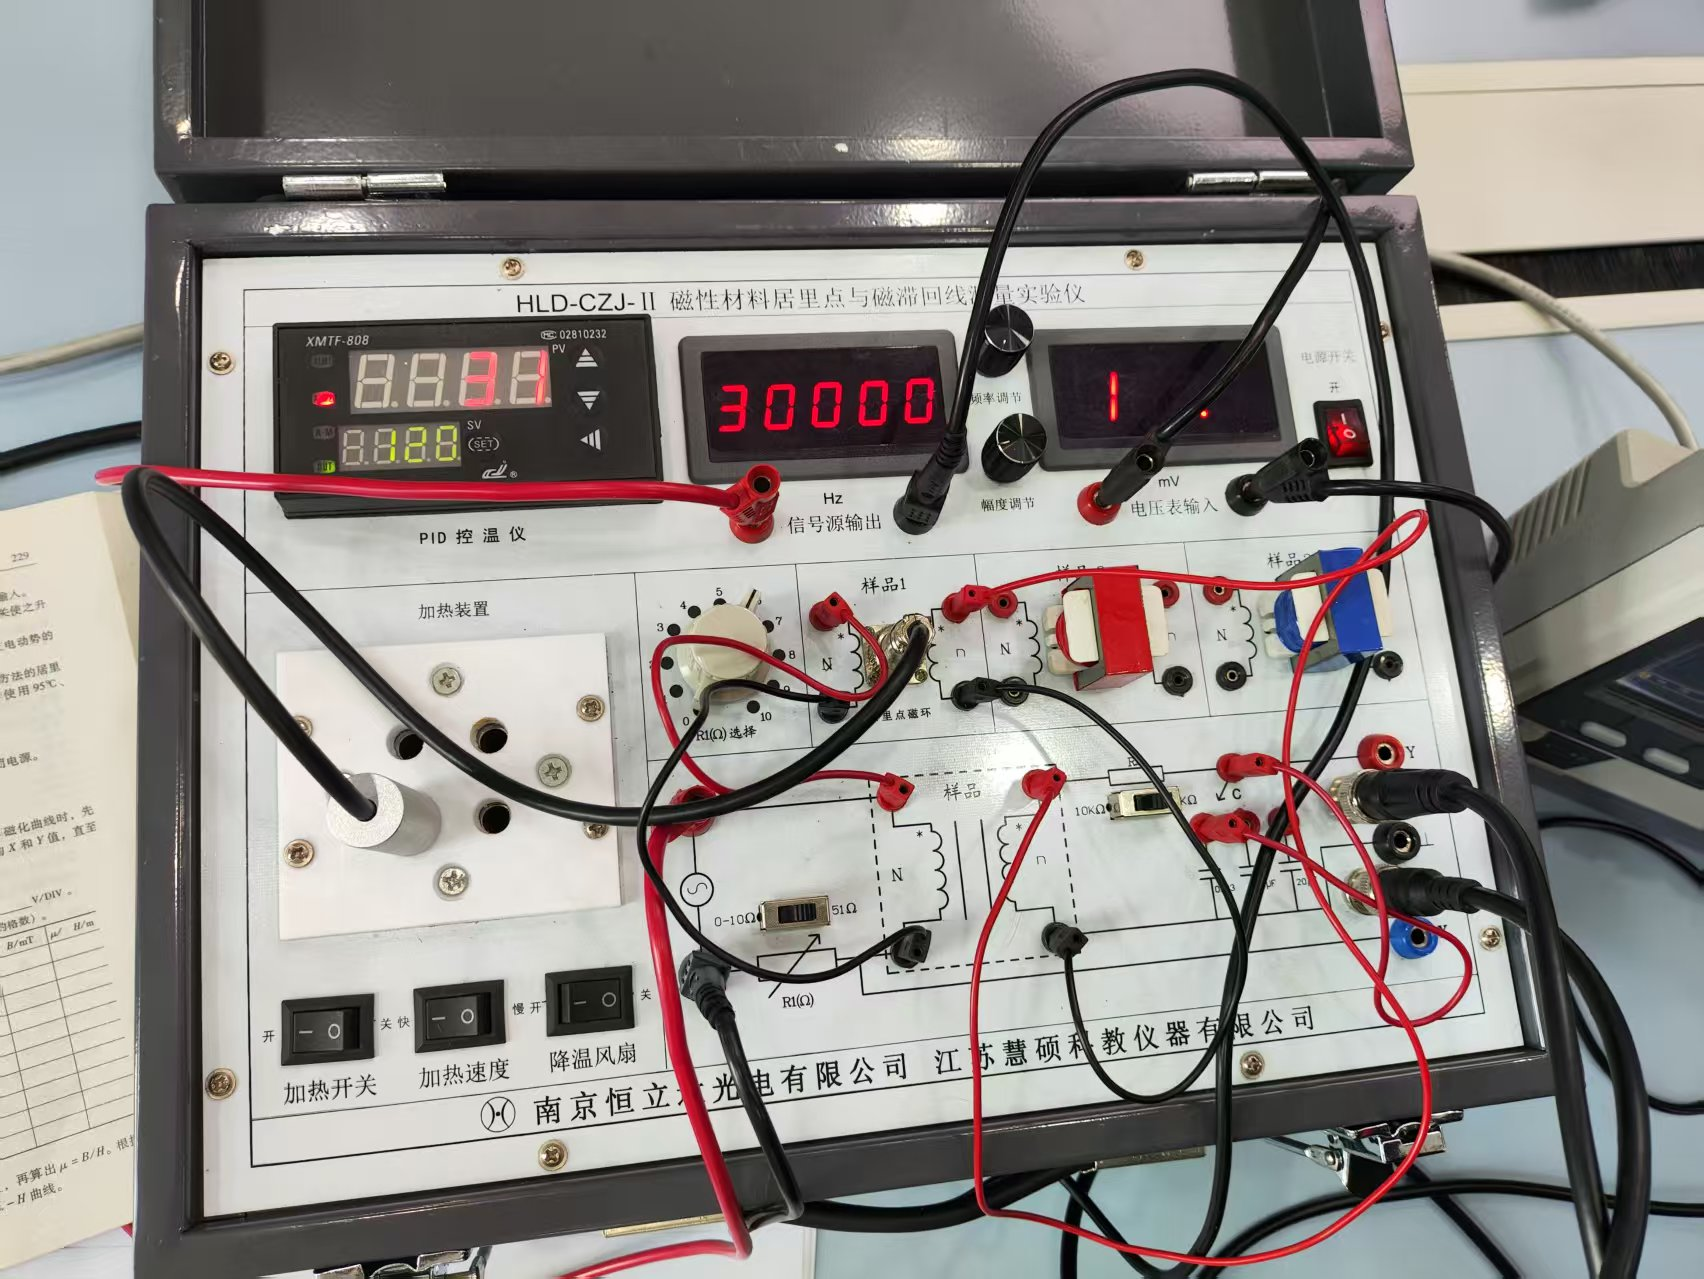
\includegraphics[width=\textwidth]{assets/实验仪.jpg}
        \caption{磁性材料居里点与磁滞回线测量实验仪}
        \label{fig:exp_funda1_left}
    \end{minipage}
    \hfill
    \begin{minipage}[t]{0.48\textwidth}
        \centering
        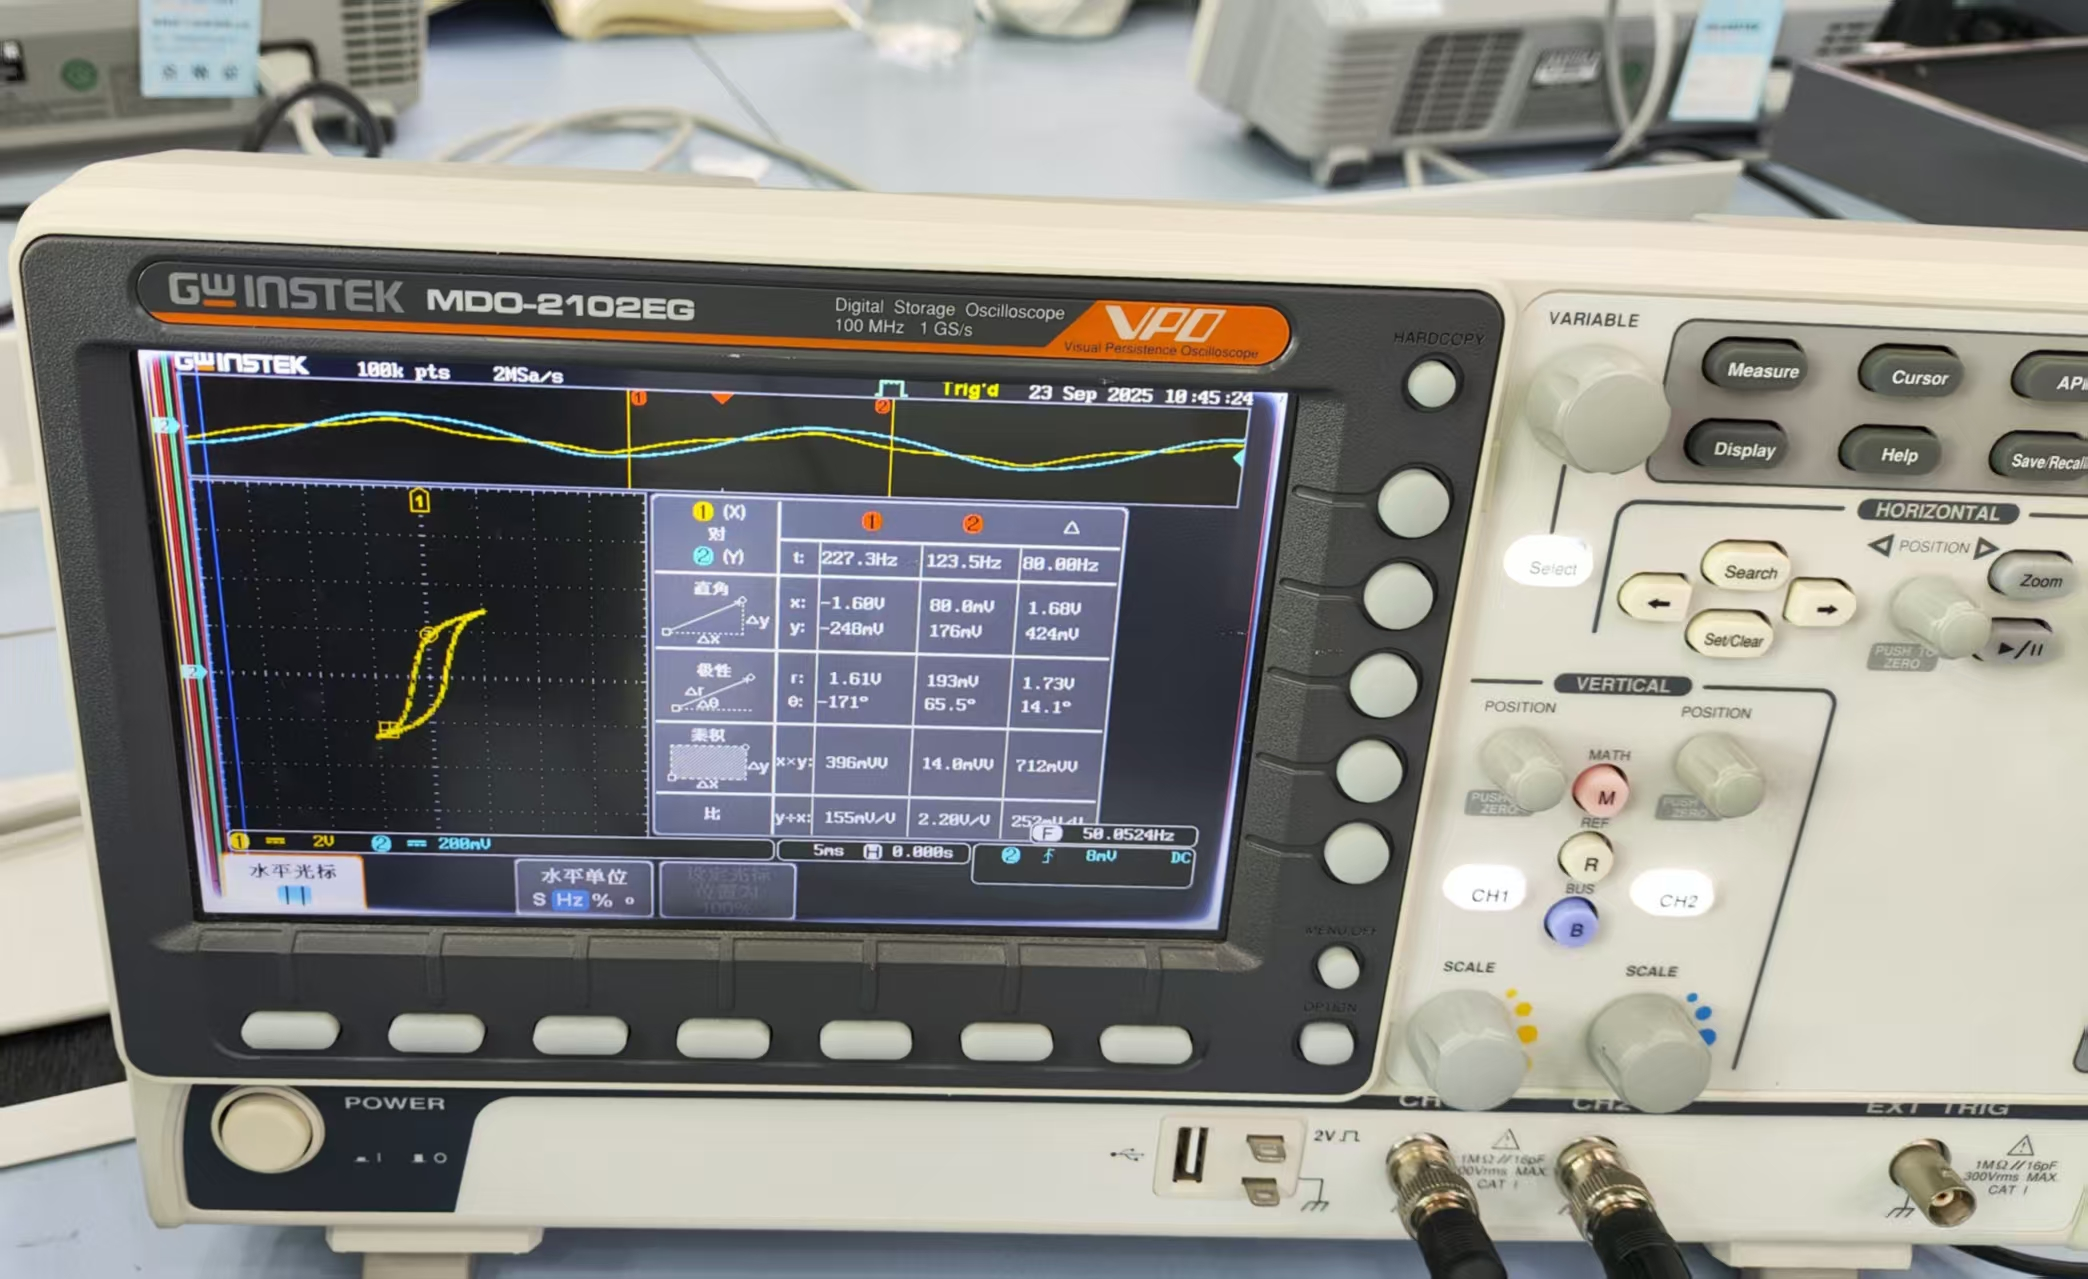
\includegraphics[width=\textwidth]{assets/示波器.jpg}
        \caption{数字示波器}
        \label{fig:exp_funda1_right}
    \end{minipage}
\end{figure}

\section{实验原理}

\subsection{铁磁材料的磁化}

铁磁材料是一种性能特殊，用途广泛的材料。铁、钴、镍及其多种合金以及含铁的氧化物（铁氧体）均属铁磁材料。其特征是在外磁场作用下能被强烈磁化，故磁导率$\mu$很高；另一特征是磁滞特性，即磁化场作用停止后，磁体仍保留一定磁化状态。

如果在由电流产生的磁场中放入铁磁材料，则磁场将明显增强，此时铁磁材料中的磁感应强度比单纯由电流产生的磁感应强度大百倍甚至千倍。铁磁材料内部的磁场强度$H$与磁感应强度$B$有如下关系：

\begin{align}
B = \mu H \tag{1}
\end{align}

对于铁磁材料而言，磁导率$\mu$并非常数，而是随$H$的变化而改变的物理量，即$\mu=\mu(H)$为非线性函数。所以$\mu$与$H$、$B$与$H$都是非线性关系。

磁滞材料的磁化过程为：其未被磁化时的状态称为去磁状态，这时若在铁磁材料上加一个由小到大的磁化场，则铁磁材料内部的磁场强度$H$与磁感应强度$B$也随之变大。但当$H$增加到一定值($H_s$)后，$B$几乎不再随$H$的增加而增加，这时磁化已达饱和。从未磁化到饱和磁化的这段磁化曲线称为材料的起始磁化曲线。

\subsection{磁滞回线}

\begin{figure}[H]
    \centering
    \begin{minipage}[t]{0.64\textwidth}
        \centering
        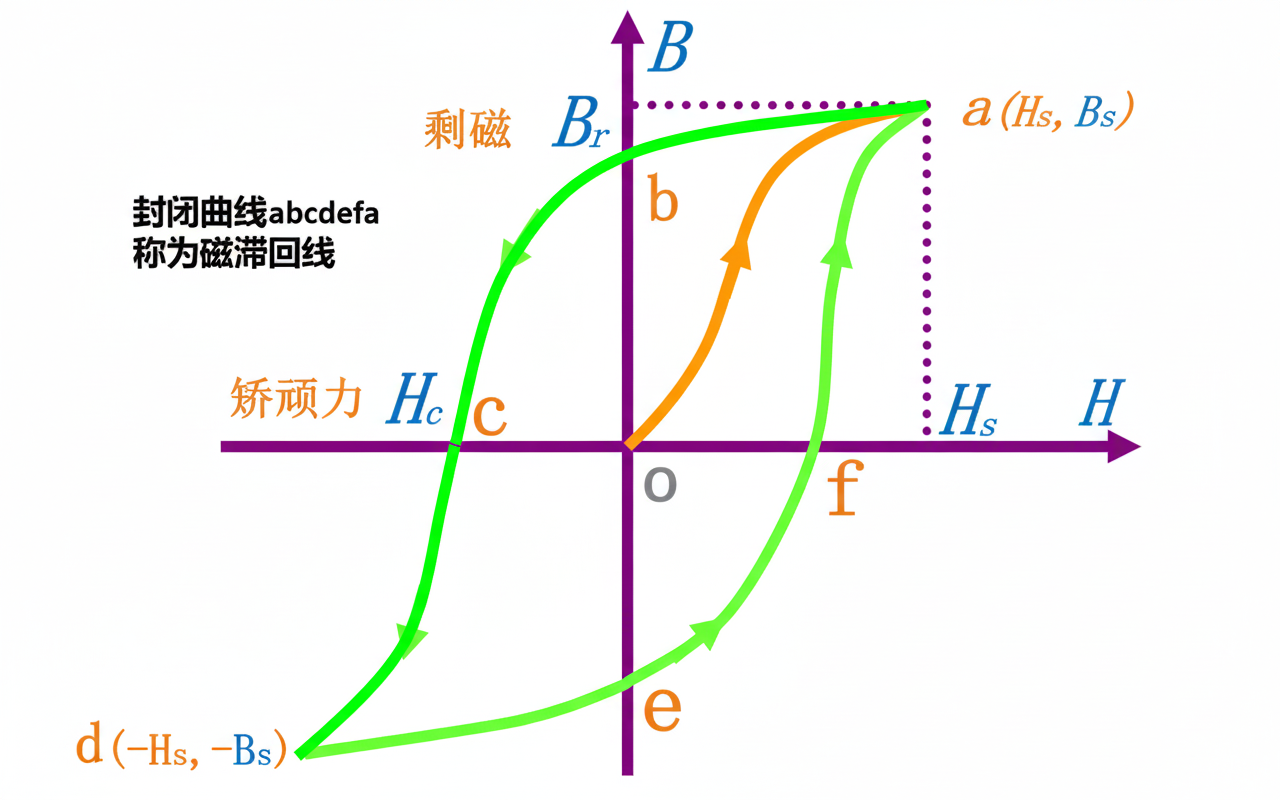
\includegraphics[width=\textwidth]{assets/磁滞回线fig.png}
        \caption{磁滞回线示意图}
        \label{fig:curie_scope_fig}
    \end{minipage}
    \hfill
    \begin{minipage}[t]{0.34\textwidth}
        \centering
        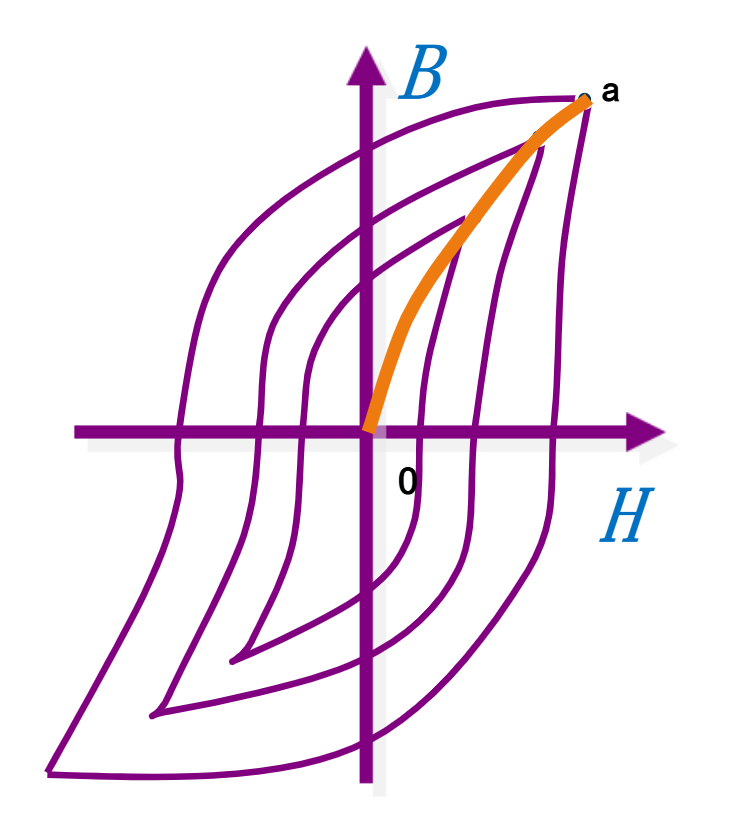
\includegraphics[width=\textwidth]{assets/基本磁化曲线fig.png}
        \caption{基本磁化曲线示意图}
        \label{fig:curie_temp_fig}
    \end{minipage}
\end{figure}


当铁磁材料的磁化达到饱和之后，如果将磁化场减小，则磁性材料内部的$B$和$H$也随之减小，但其减小的过程并不沿着磁化时的OS段退回。当磁化场撤消，$H=0$时，磁感应强度仍然保持一定数值$B_r$，称为剩磁（剩余磁感应强度）。

若要使被磁化的铁磁材料的磁感应强度$B$减小到0，必须加上一个反向磁场并逐步增大。当铁磁材料内部反向磁场强度增加到$H=-H_c$时，磁感应强度$B$才是0，达到退磁。$H_c$称为矫顽力。当$H$按$O \to H_s \to -H_s \to O \to H_s$的顺序变化时，$B$相应地按$O \to B_s \to B_r \to O \to B_s$的顺序变化。上述变化过程所形成的封闭曲线称为磁滞回线。

由上可得以下结论：当$H=0$时，$B \neq 0$，这说明铁磁材料还残留一定的磁感应强度，称之为剩磁；若要使铁磁材料完全退磁，即$B=0$，必须加一个反向磁场$-H_c$，这个磁场强度$H_c$称为该铁磁材料的矫顽力；$B$的变化始终落后于$H$的变化，即$H$减为0时$B$不为0，$H$反向到一定值时$B$才为0，这称为磁滞现象；由磁滞回线的图象可知，对应$H$的某一数值，铁磁材料内的$B$值可能不同，$B$值与铁磁材料过去的磁化经历有关。

由于铁磁材料磁化过程的不可逆性及具有剩磁的特点，在测定磁化曲线和磁滞回线时，首先必须将铁磁材料预先退磁，以保证外加磁场$H=0$时$B=0$；其次，磁化电流在实验过程中只允许单调增加或减少，不能瞬时增减。我们把原点O和各个磁滞回线的顶点所连成的曲线称为铁磁材料的基本磁化曲线。不同的铁磁材料其基本磁化曲线是不同的。为了使样品的磁特性可以重复出现，在测量前必须进行退磁，以消除样品中的剩余磁性。

\subsection{示波器显示B-H曲线的原理}

本实验研究的铁磁材料（待测样品）为EI型硅钢片，$N$为初级励磁绕组，$n$为用来测量磁感应强度$B$而设置的次级测量绕组。$R_1$为励磁电流取样电阻，把电流转换为电压。设通过$N$的交流励磁电流为$i_1$。

根据安培环路定律，样品的磁化场强为：
\begin{align}
H = \frac{Ni_1}{L} \tag{2}
\end{align}

式中，$L$为样品的平均磁路长度。因为$i_1 = \frac{u_1}{R_1}$，所以：
\begin{align}
H = \frac{N}{L}\frac{u_1}{R_1} = \frac{Nu_1}{LR_1} \tag{3}
\end{align}

式中的$N$、$L$、$R_1$均为已知常数，所以由$u_1$可确定$H$。

在交变磁场下，样品的磁感应强度瞬时值$B$是由测量绕组$n$和$R_2$、$C_2$电路给定的，根据法拉第电磁感应定律，由于样品中的磁通$\phi$的变化，在测量线圈中产生的感生电动势的大小为：
\begin{align}
\varepsilon_2 = -n\frac{d\phi}{dt}
\end{align}

\begin{align}
\phi = \frac{1}{n}\int\varepsilon_2 dt
\end{align}

\begin{align}
B = \frac{\phi}{S} = \frac{1}{nS}\int\varepsilon_2 dt \tag{4}
\end{align}

$S$为样品的截面积。

如果忽略自感电动势和电路损耗，则回路方程为：
\begin{align}
\varepsilon_2 = i_2R_2 + u_C
\end{align}

式中，$i_2$为感生电流，$u_C$为积分电容$C$两端电压。设在$\Delta t$时间内，$i_2$向电容$C$的充电电量为$Q$，则：
\begin{align}
u_C = \frac{Q}{C} \tag{5}
\end{align}

所以：
\begin{align}
\varepsilon_2 = i_2R_2 + \frac{Q}{C} \tag{6}
\end{align}

如果选取足够大的$R_2$和$C$使$i_2R_2 \gg \frac{Q}{C}$，则：
\begin{align}
\varepsilon_2 \approx i_2R_2 \tag{7}
\end{align}

因为：
\begin{align}
i_2 = \frac{dQ}{dt} = C\frac{du_C}{dt} \tag{8}
\end{align}

所以：
\begin{align}
\varepsilon_2 = CR_2\frac{du_C}{dt} \tag{9}
\end{align}

由式(4)、(9)两式可得：
\begin{align}
B = \frac{CR_2}{nS}u_C \tag{10}
\end{align}

上式中$C$、$R_2$、$n$和$S$均为已知常数，所以由$u_C$可确定$B$。

综上所述，$u_1(u_H)$和$u_C(u_B)$分别加到示波器的"X输入"和"Y输入"便可观察样品的动态磁滞回线；接上数字电压表则可以直接测出$u_1(u_H)$和$u_C(u_B)$的值，即可绘制出B-H曲线，通过计算可测定样品的饱和磁感应强度$B_s$、剩磁$B_r$、矫顽力$H_c$、磁滞损耗以及磁导率$\mu$等参数。

\subsection{居里点测量原理}

在磁环上分别绕线圈$N$、$n$，并在$N$线圈上通励磁电流，则$n$线圈上感应电动势的有效值为：
\begin{align}
\varepsilon_{eff} = 4.44fn\Phi_m \tag{11}
\end{align}

式中，$f$为频率；$n$为线圈匝数；4.44为仪器常数；$\Phi_m$为最大磁通。

\begin{align}
\Phi_m = B_mS \tag{12}
\end{align}

$S$为磁环的截面积；$B_m$为最大磁感应强度，即磁感应强度正弦变化的幅值。又因为：
\begin{align}
H = B/\mu \tag{13}
\end{align}

$\mu$是磁导率，在SI制中单位为H/m。把式(12)、(13)代入式(11)，得：
\begin{align}
\varepsilon_{eff} = 4.44fnS\mu H_m \tag{14}
\end{align}

$H_m$是磁场强度的幅值，当励磁电流稳定成正弦变化时，则$H_m$恒定。即得：
\begin{align}
\varepsilon_{eff} \propto \mu \tag{15}
\end{align}

铁磁材料的$\mu$通常高达$10^4$数量级，而顺磁材料$\mu \approx 1$，所以温度升高到居里点$T_c$附近时，感应电动势会急剧下降。显然，我们完全可用测出的$\varepsilon_{eff}-T$曲线来确定温度$T_c$。具体地讲，在$\varepsilon_{eff}-T$曲线斜率最大处作切线，其与横坐标轴相交的一点即为$T_c$。这是因为在居里点时，铁磁材料的磁性发生突变，所以要在斜率最大处作切线。

\section{实验步骤}

观察EI型硅钢片磁滞回线图形时，先选择样品2进行实验，连接电路，取样电阻$R_1$的选择开关置于0~100Ω挡，多挡开关挡位置于6Ω左右，$R_2$的选择开关置于10kΩ，积分电容$C$选择10$\mu$F。调示波器显示工作方式为X-Y方式，即图示仪方式。示波器X输入为AC方式，测量采样电阻$R_1$的电压；示波器Y输入为DC方式，测量积分电容$C$的电压。接通示波器和实验平台的电源，信号源输出频率调到50Hz，幅度先调为0V，此时示波器上应显示居中的亮点。调节信号源幅度旋钮逐渐增加磁化电流使示波器显示出磁滞回线现象（稍后，B值缓慢增加达到饱和）。改变示波器上X、Y灵敏度使示波器显示出典型美观的磁滞回线图形。如不在中间，可调节示波器的X、Y位移旋钮使图形清晰、对称、居中。保持信号源幅度旋钮逐渐减少磁化电流，观察磁滞回线由大变小直至缩成一点，此为退磁过程。

测绘铁磁材料的基本磁化曲线和饱和磁滞回线时，在直角坐标纸上以$u_H(H)$为横坐标，以$u_B(B)$为纵坐标建立坐标系，原点位于纸的中央，坐标纸刻度与示波器屏幕上的刻度形成对应关系（图线清楚可适当放大比例）。从0开始逐渐增加磁化电流使磁滞回线由小到大直至饱和，选择10个适当的点停下来，读取它们的X、Y坐标值，并把磁滞回线的顶点位置描记在坐标纸上，平滑地连接这些点即得到基本磁化曲线。在同一坐标系里先描点再连线，描绘出完整的饱和磁滞回线。注意几个关键值$B_s$、$B_r$、$H_c$的坐标要尽量准确。记录示波器X、Y轴灵敏度的值（V/DIV），示波器的灵敏度在上述实验过程中必须保持不变。

通过观察磁滞回线消失时的温度测定居里点时，将居里点探测样品的探头端插入加热片，插头端插入面板上样品1的插座，选择$R_1 = 510$Ω，$R_2 = 1$kΩ，$C=0.33\mu$F，信号源频率为30kHz，幅度16V$_{p-p}$。$u_H$和$u_B$分别接示波器的"X输入"和"Y输入"，地为公共端。打开实验仪和示波器电源开关，此时面板上加热开关为关闭状态，适当调节示波器，在屏幕上显示磁滞回线。将\textbf{加热开关打开，加热速度选择快}。通过表头预设温度120℃，对样品进行加热。在此过程中观察示波器上的磁滞回线，记下磁滞回线消失时（变为一条直线）显示的温度值，此即测到的居里点温度。测量完成后将加热开关关闭，打开降温风扇使加热片降温。

\section{数据记录与处理}

实验中使用示波器X轴放大倍数为4，对磁性材料的磁化特性进行了系统测量。

\subsection{磁滞回线特征点测量数据}

对磁滞回线的特征点进行了精确测量，数据记录如下表所示：

\begin{table}[H]
\centering
\caption{磁滞回线特征点测量数据}
\begin{tabular}{|c|c|c|c|}
\hline
测量点 & $u_H$ (V) & $u_B$ (mV) & 备注 \\
\hline
a & 2.08 & 288 & 第一象限饱和点 \\
\hline
b & 0.00 & 176 & 正剩磁点 \\
\hline
c & -0.640 & 0.00 & 负矫顽力点 \\
\hline
d & -2.08 & -272 & 第三象限饱和点 \\
\hline
e & 0.00 & -144 & 负剩磁点 \\
\hline
f & 0.560 & 0.00 & 正矫顽力点 \\
\hline
\end{tabular}
\end{table}

\begin{table}[H]
\centering
\caption{磁滞回线各段中点测量数据}
\begin{tabular}{|c|c|c|c|}
\hline
线段 & $u_H$ (V) & $u_B$ (mV) & 位置描述 \\
\hline
ab段中点 & 0.720 & 232 & 上升段中点 \\
\hline
bc段中点 & -0.480 & 80.0 & 下降段中点 \\
\hline
cd段中点 & -0.880 & -112 & 负向上升段中点 \\
\hline
de段中点 & -0.640 & -208 & 负向下降段中点 \\
\hline
ef段中点 & 0.320 & -80.0 & 回升段中点 \\
\hline
fa段中点 & 0.800 & 128 & 正向恢复段中点 \\
\hline
\end{tabular}
\end{table}

\subsection{基本磁化曲线测量数据}

基本磁化曲线上10个关键点的电压测量值记录如下表：

\begin{table}[H]
\centering
\caption{基本磁化曲线测量数据}
\begin{tabular}{|c|c|c|}
\hline
测量点序号 & $u_H$ (V) & $u_B$ (mV) \\
\hline
1 & 1.50 & 250 \\
\hline
2 & 1.22 & 228 \\
\hline
3 & 1.03 & 206 \\
\hline
4 & 0.860 & 184 \\
\hline
5 & 0.720 & 152 \\
\hline
6 & 0.620 & 132 \\
\hline
7 & 0.520 & 104 \\
\hline
8 & 0.440 & 80.0 \\
\hline
9 & 0.360 & 56.0 \\
\hline
10 & 0.240 & 28.0 \\
\hline
\end{tabular}
\end{table}

\subsection{实验结果图像}

根据测量数据，利用MATLAB软件绘制了磁滞回线和基本磁化曲线，如图1和图2所示。

\begin{figure}[H]
    \centering
    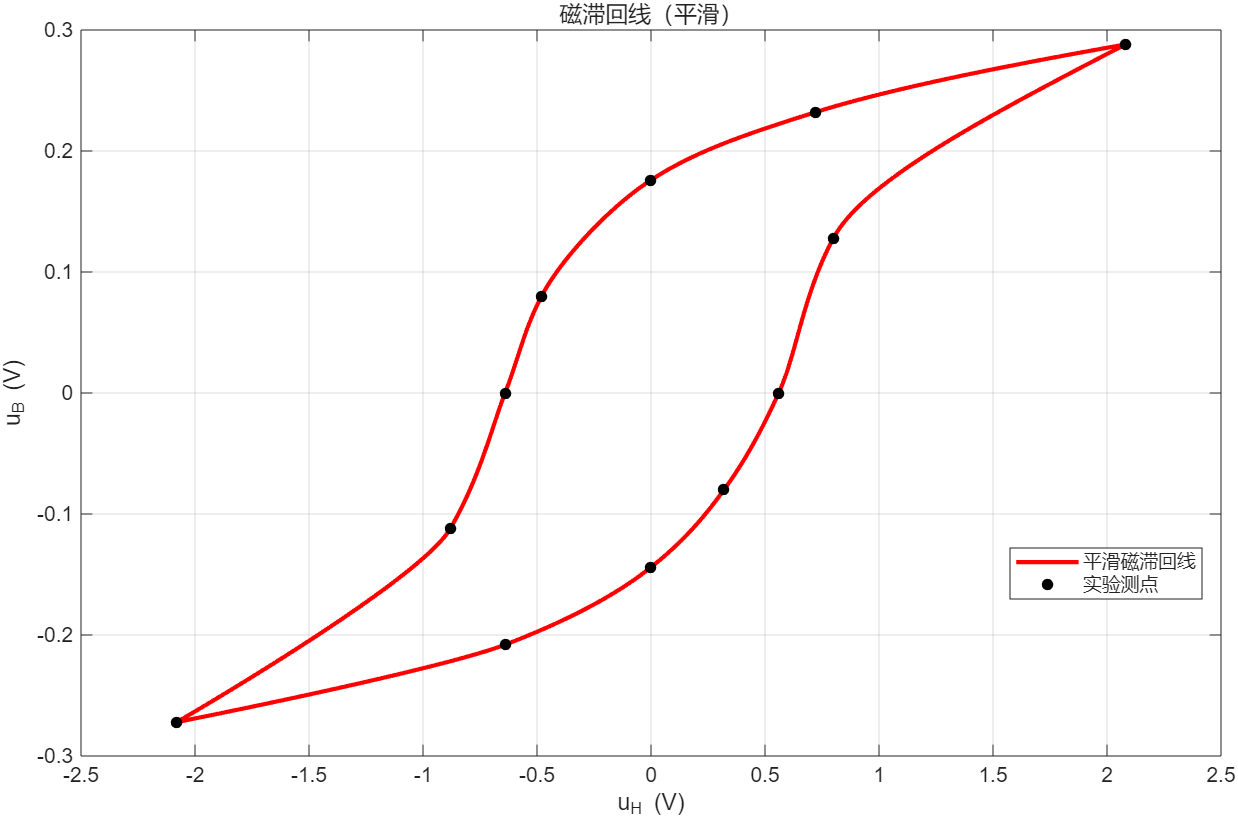
\includegraphics[width=0.8\textwidth]{assets/磁滞回线.png}
    \caption{磁滞回线（平滑）}
    \label{fig:hysteresis}
\end{figure}

\begin{figure}[H]
    \centering
    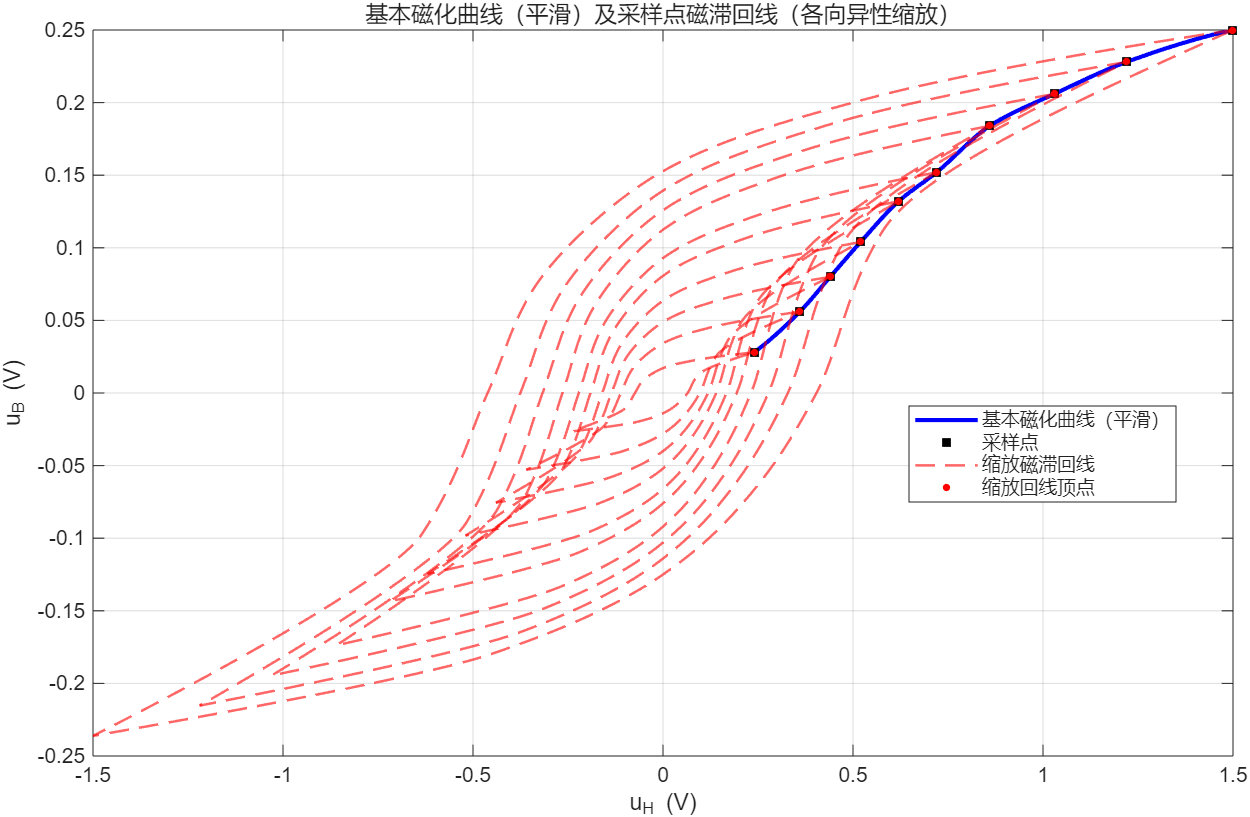
\includegraphics[width=0.8\textwidth]{assets/基本磁化曲线.png}
    \caption{基本磁化曲线（平滑）及采样点磁滞回线（各向异性缩放）}
    \label{fig:magnetization}
\end{figure}

\subsection{居里点测量结果}

通过观察磁滞回线在温度变化过程中的消失现象，测得样品的居里点温度为104℃。实验过程中，随着温度的不断升高，磁滞回线逐渐变窄，直至完全消失变为一条直线，标志着材料从铁磁性转变为顺磁性。

\begin{figure}[H]
    \centering
    \begin{minipage}[t]{0.48\textwidth}
        \centering
        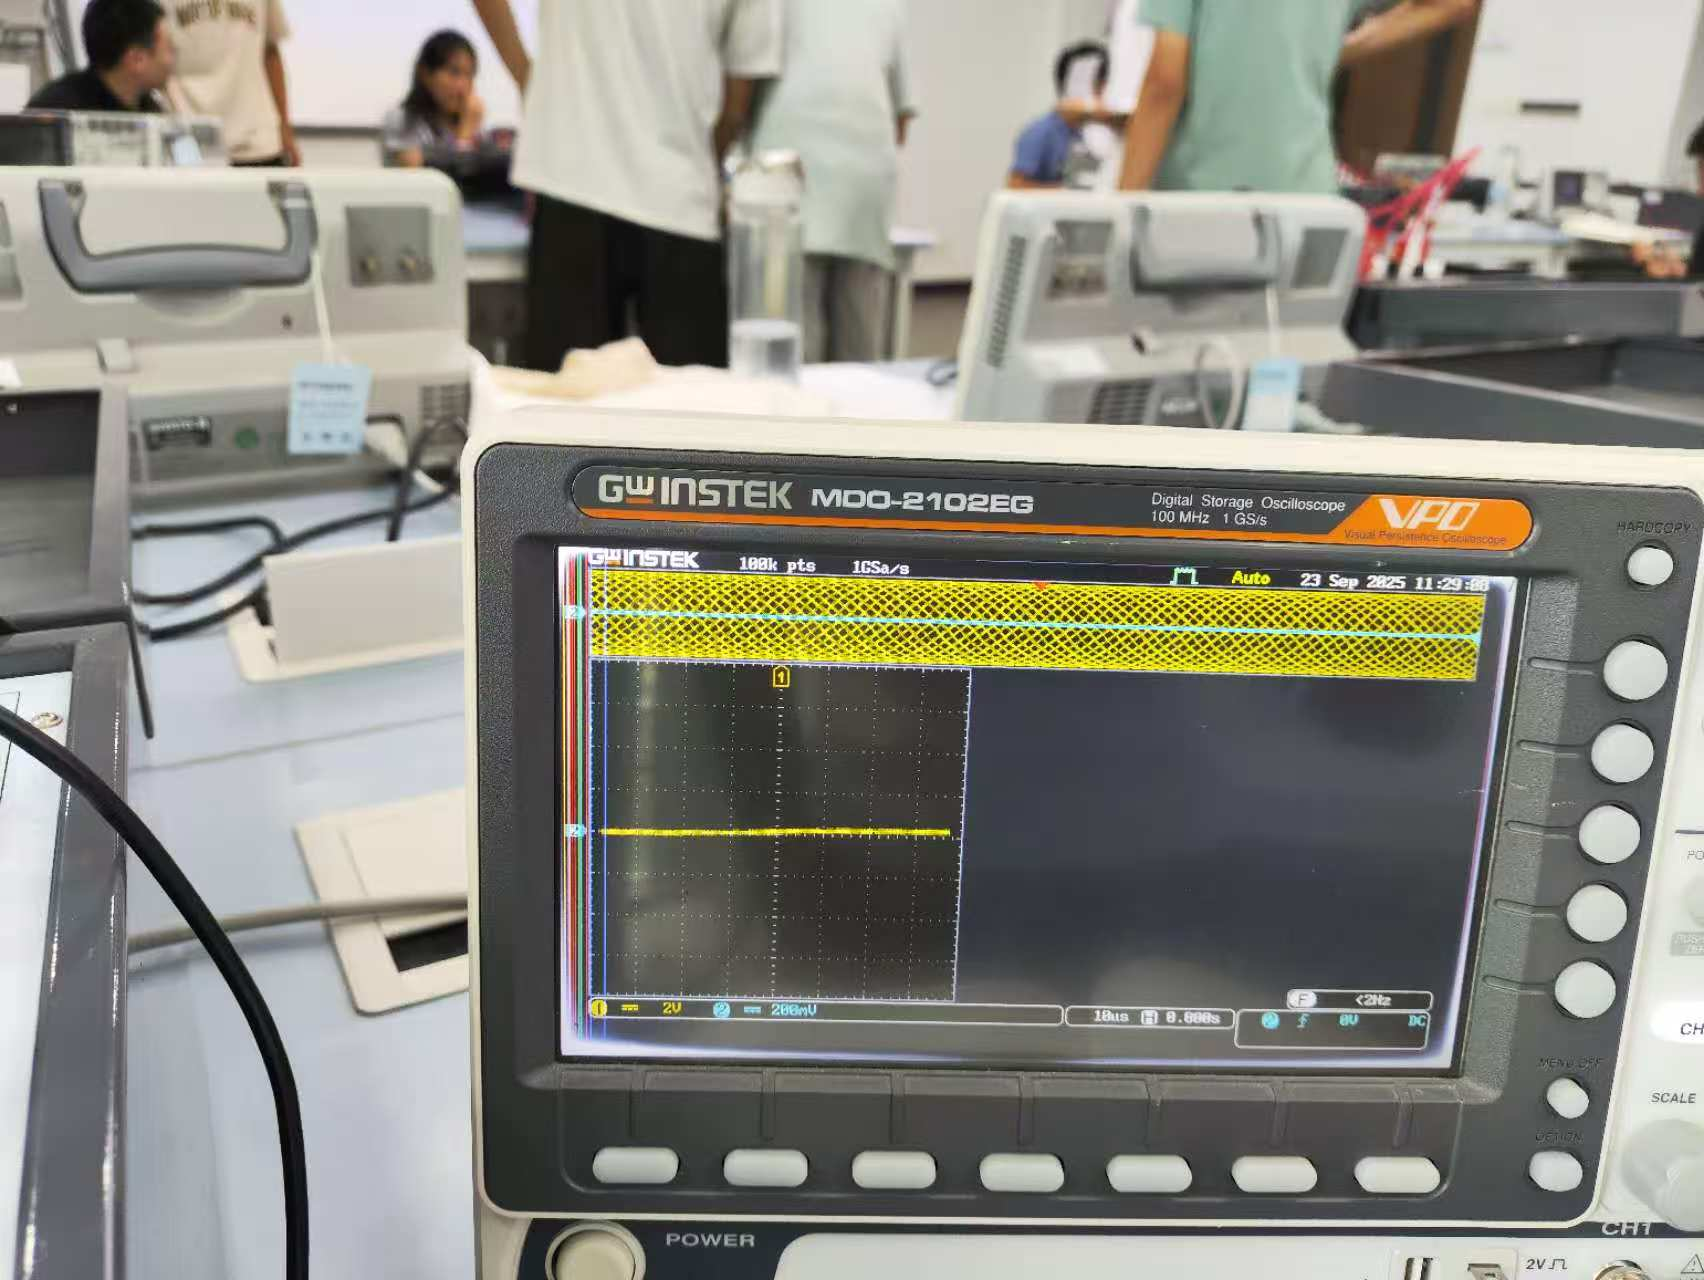
\includegraphics[width=\textwidth]{assets/居里点回线.jpg}
        \caption{居里点时磁滞回线消失现象}
        \label{fig:curie_scope}
    \end{minipage}
    \hfill
    \begin{minipage}[t]{0.48\textwidth}
        \centering
        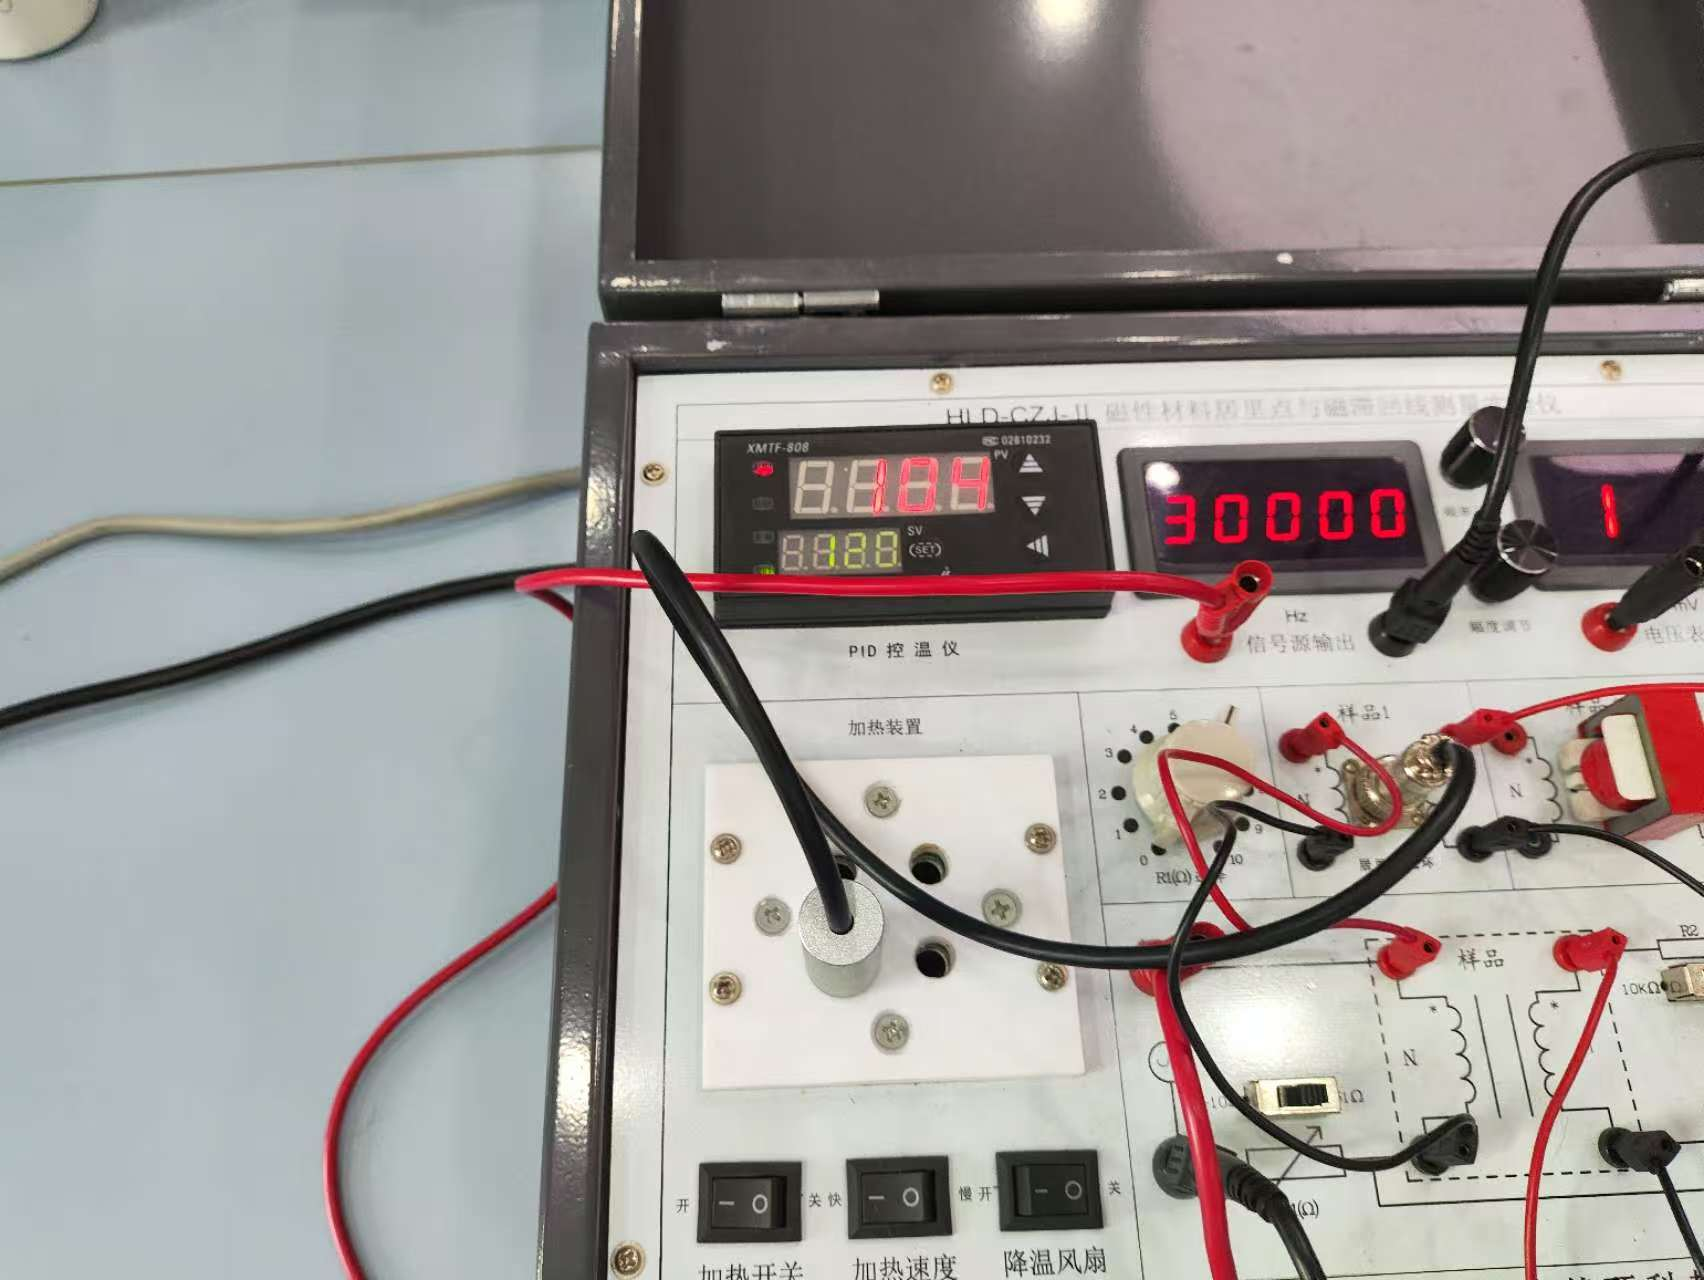
\includegraphics[width=\textwidth]{assets/居里点温度.jpg}
        \caption{居里点温度}
        \label{fig:curie_temp}
    \end{minipage}
\end{figure}

如图\ref{fig:curie_scope}所示，当温度达到居里点时，示波器上原本清晰的磁滞回线完全消失，变为一条水平直线，这表明样品已失去铁磁性。图\ref{fig:curie_temp}显示了实验过程中温度控制面板的状态，通过PID控制器精确控制样品温度，确保测量的准确性。实验结果表明，该铁氧体样品的居里点温度为104℃，这一结果与理论预期相符。

\appendix

\section{数据处理MATLAB代码}

\begin{lstlisting}[style=Matlab-boxed,caption={磁滞回线与基本磁化曲线数据处理代码}]
clear; clc; close all;
%% Raw Data
x_hyst = [ 2.08, 0.72, 0.00, -0.48, -0.64, -0.88, -2.08, -0.64, ...
           0.00, 0.32, 0.56, 0.80, 2.08]; % V
y_hyst = [ 0.288, 0.232, 0.176, 0.080, 0.000, -0.112, -0.272, -0.208, ...
           -0.144, -0.080, 0.000, 0.128, 0.288]; % V

% 平滑模板回线 pchip
t = 1:numel(x_hyst);
tt = linspace(1, numel(x_hyst), 600);
x_hyst_s = pchip(t, x_hyst, tt);
y_hyst_s = pchip(t, y_hyst, tt);

% a 点
x_a = 2.08; % V
y_a = 0.288; % V

%% 基本磁化曲线(10 点)
x_mag = [1.50, 1.22, 1.03, 0.86, 0.72, 0.62, 0.52, 0.44, 0.36, 0.24]; % V
y_mag = [0.250, 0.228, 0.206, 0.184, 0.152, 0.132, 0.104, 0.080, 0.056, 0.028]; % V

xx = linspace(min(x_mag), max(x_mag), 400);
yy = pchip(x_mag, y_mag, xx);

%% 磁滞回线（平滑）
figure('Color','w');
plot(x_hyst_s, y_hyst_s, 'r-', 'LineWidth', 2); hold on;
plot(x_hyst, y_hyst, 'ko', 'MarkerFaceColor','k', 'MarkerSize',5);
grid on;
xlabel('u_H (V)'); ylabel('u_B (V)');
title('磁滞回线（平滑）');
legend('平滑磁滞回线','实验测点','Location','best');

%% 基本磁化曲线 + 各采样点的小磁滞回线
figure('Color','w');
plot(xx, yy, 'b-', 'LineWidth', 2); hold on;
plot(x_mag, y_mag, 'ks', 'MarkerFaceColor','k', 'MarkerSize',5);

alphaVal = 0.6; lw = 1.2;
for i = 1:numel(x_mag)
    scale_x = x_mag(i) / x_a;
    scale_y = y_mag(i) / y_a;
    xs = scale_x * x_hyst_s;
    ys = scale_y * y_hyst_s;
    p = plot(xs, ys, 'r--', 'LineWidth', lw);
    p.Color(4) = alphaVal;
    
    % 缩放后的 a 点
    xa_tip = scale_x * x_a;
    ya_tip = scale_y * y_a;
    plot(xa_tip, ya_tip, 'ro', 'MarkerFaceColor','r', 'MarkerSize',3);
end

grid on;
xlabel('u_H (V)'); ylabel('u_B (V)');
title('基本磁化曲线（平滑）及采样点磁滞回线（各向异性缩放）');
legend('基本磁化曲线（平滑）','采样点','缩放磁滞回线','缩放回线顶点','Location','best');

%% 居里点输出
Tc = 104;
fprintf('测得居里点温度: %d °C\n', Tc);
\end{lstlisting}

\end{document}
